Numerical simulations are crucial in physics and astronomy for studying complex systems of interacting particles, such as galaxies and the Universe's large-scale structure, where analytical solutions are often impractical due to complexity and nonlinearity \citep{1981csup.book.....H, 1985ApJS...57..241E, 2005Natur.435..629S, 2005MNRAS.364.1105S}. This section provides an overview of $N$-body simulations commonly used in cosmology.

In cosmology and astrophysics, simulation can be grouped into two main categories: dark matter-only simulations and hydrodynamical simulations. 

Dark matter simulations are used to study the large-scale structure of the universe, the formation of dark matter halos, and the evolution of dark matter particles under the influence of gravity. Since dark matter is effectively collisionless and interacts primarily through gravity, it can be modeled as a collection of particles that evolve under the influence of gravitational forces \citep{1985ApJS...57..241E}. 

Hydrodynamical simulations, on the other hand, include the effects of gas dynamics, star formation, and feedback processes from supernovae and active galactic nuclei (AGN) \citep{1989ApJS...70..419H, 2005Natur.435..629S, 2005MNRAS.364.1105S}. These simulations are more computationally expensive and require additional physics beyond gravity, such as hydrodynamics, radiative transfer, and chemistry.

Since the 1980s, numerical cosmology has developed algorithms to mitigate the computational challenges posed by long-range gravitational interactions by reducing global communication across the computational domain. Key algorithms include mesh-based methods, tree codes, and multipole expansions~\citep{1981csup.book.....H}. Figure~\ref{fig:particle-count} displays the number of particles used in selected $N$-body simulations employing these techniques. Symbols and colors indicate the gravitational solvers: particle-particle-particle-mesh (P$^3$M) and adaptive P$^3$M (AP$^3$M); parallel or vectorized P$^3$M; Tree codes; TreePM; and particle-mesh methods with adaptive mesh refinement (PM AMR).

Advancements in algorithms and software optimization have increased the number of particles in cosmological simulations beyond what direct summation methods allow. Since 1990, gravity-only simulations have exhibited a super-exponential growth trend, indicated by the quadratic regression in Figure~\ref{fig:particle-count}, reflecting significant methodological innovations beyond hardware improvements~\citep{leclercq2020}.

\begin{figure} \centering 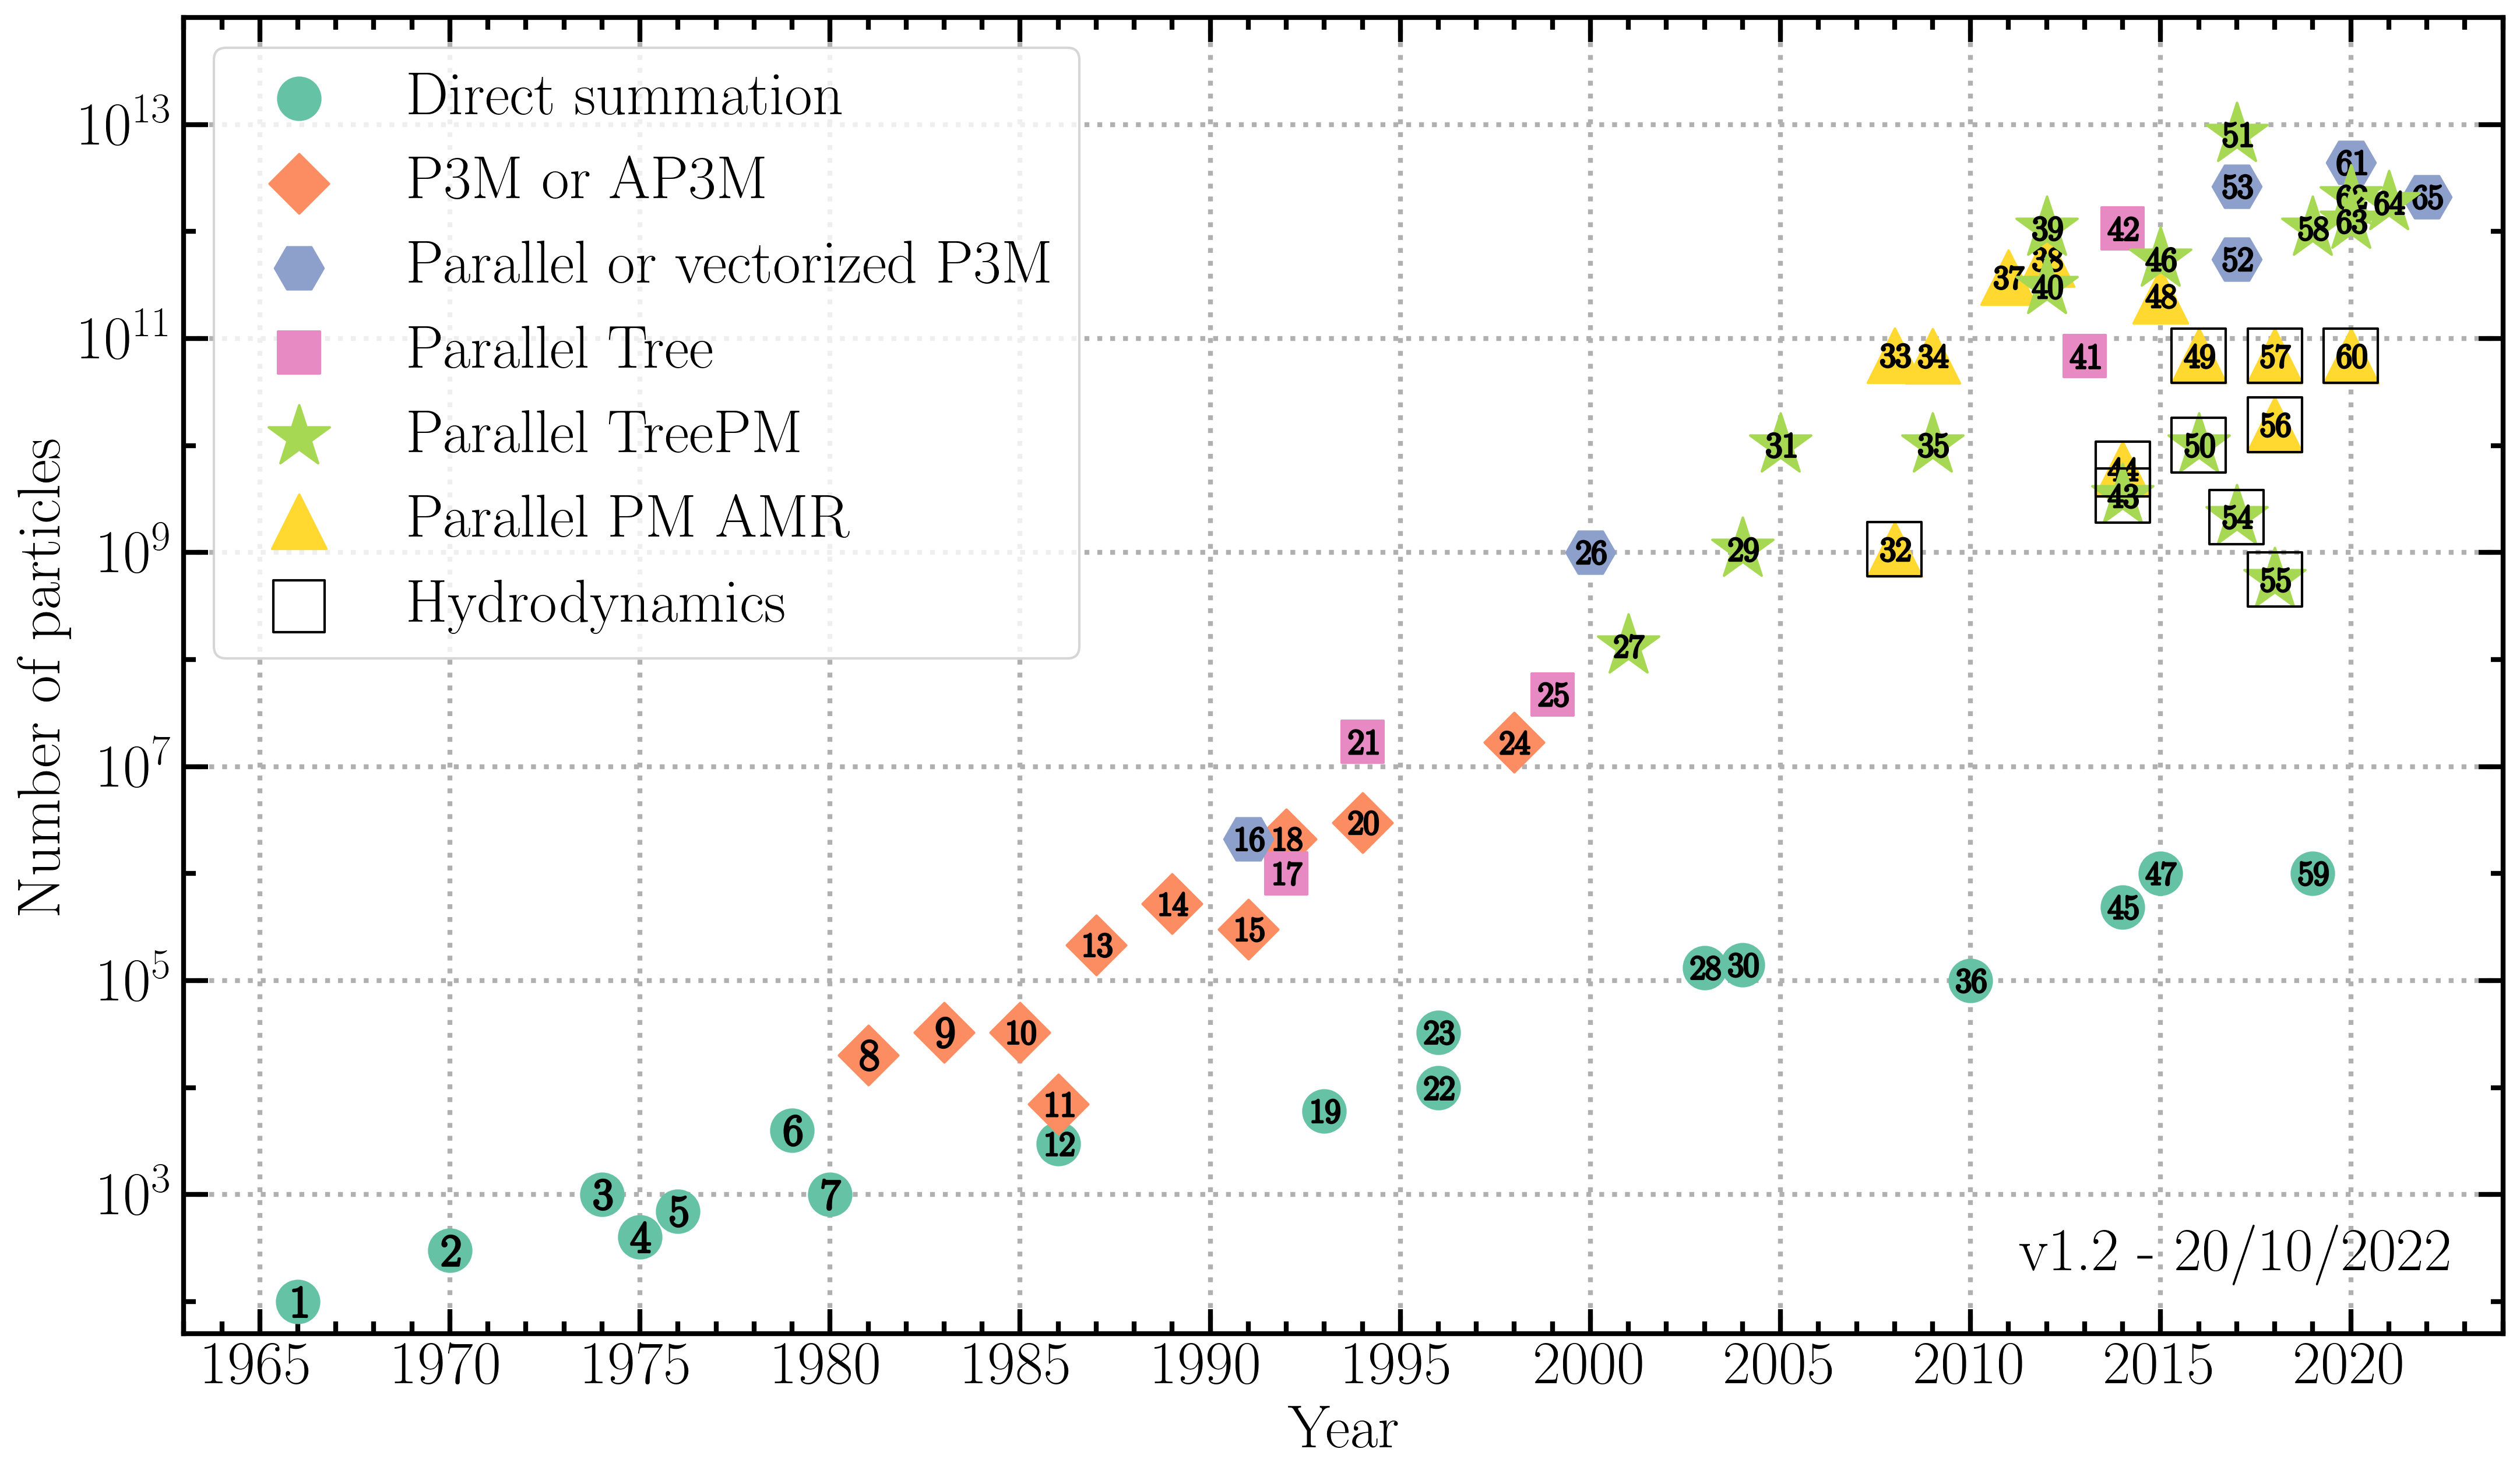
\includegraphics[width=\textwidth]{figures/Moore_law_cosmosims.png} \caption[Evolution of the number of particles used in $N$-body simulations]{Evolution of the number of particles used in $N$-body simulations as a function of the year of publication~\citep{leclercq2020}. The symbols and colors indicate the gravitational solver employed: P$^3$M and adaptive P$^3$M (AP$^3$M); parallel or vectorized P$^3$M; Tree codes; TreePM; and particle-mesh methods with adaptive mesh refinement (PM AMR). Hydrodynamic simulations are represented by black squares.} \label{fig:particle-count} \end{figure}

\section{Initial Condition Generation}
As we have seen in Section~\ref{sec:initial_conditions}, the primodial power spectrum $P(k)$ is a key ingredient in generating initial conditions for cosmological simulations. Based on the linear power spectrum, we will review the process of generating initial conditions for $N$-body simulations.

\subsection{Initial Density Field}
To generate the initial density field for the simulations, we express the density contrast $\delta(\mathbf{x})$ in terms of its Fourier components:
\begin{equation}
    \delta(\mathbf{x}) = \int \frac{d^3k}{(2\pi)^3} \tilde{\delta}(\mathbf{k}) e^{i\mathbf{k} \cdot \mathbf{x}}.
\end{equation}
Assuming a Gaussian random field, each Fourier mode $\tilde{\delta}(\mathbf{k})$ is a complex Gaussian random variable with zero mean and variance $P(k)$:
\begin{align}
    \tilde{\delta}(\mathbf{k}) &= A(\mathbf{k}) + i B(\mathbf{k}), \\
    \langle A(\mathbf{k}) \rangle &= \langle B(\mathbf{k}) \rangle = 0, \\
    \langle A(\mathbf{k}) A(\mathbf{k}') \rangle &= \langle B(\mathbf{k}) B(\mathbf{k}') \rangle = \frac{1}{2} P(k) \delta_D(\mathbf{k} - \mathbf{k}'), \\
    \langle A(\mathbf{k}) B(\mathbf{k}') \rangle &= 0,
\end{align}
where $A(\mathbf{k})$ and $B(\mathbf{k})$ are real Gaussian random variables, and $\delta_D$ is the Dirac delta function.

\subsection{Initial Displacement Field}
The initial displacement field $\boldsymbol{\Psi}(\mathbf{q})$ relates the Lagrangian coordinates $\mathbf{q}$ to the Eulerian coordinates $\mathbf{x}$:
\begin{equation}
    \mathbf{x}(\mathbf{q}) = \mathbf{q} + \boldsymbol{\Psi}(\mathbf{q}).
\end{equation}
The displacement field is proportional to the gradient of the gravitational potential $\Phi(\mathbf{q})$:
\begin{equation}
    \boldsymbol{\Psi}(\mathbf{q}) = - \nabla \Phi(\mathbf{q}),
\end{equation}
where the potential satisfies Poisson's equation:
\begin{equation}
    \nabla^2 \Phi(\mathbf{q}) = \delta(\mathbf{q}).
\end{equation}
The first order solution to the displacement field is given by the Zel'dovich approximation \citep{1970A&A.....5...84Z}:
\begin{align}
    -k^2 \tilde{\Phi}(\mathbf{k}) &= \tilde{\delta}(\mathbf{k}), \\
    \tilde{\boldsymbol{\Psi}}(\mathbf{k}) &= i \mathbf{k} \tilde{\Phi}(\mathbf{k}) = i \mathbf{k} \frac{\tilde{\delta}(\mathbf{k})}{k^2}, \\
    \boldsymbol{\Psi}(\mathbf{q}) &= \int \frac{d^3k}{(2\pi)^3} i \mathbf{k} \frac{\tilde{\delta}(\mathbf{k})}{k^2} e^{i\mathbf{k} \cdot \mathbf{q}}.
\end{align}

\subsection{Initial Velocities}
The initial velocities of particles are derived from the time derivative of the displacement field. The velocities are given by \citep{1985ApJS...57..241E}:
\begin{align}
    \mathbf{v}(\mathbf{q}) &= a H f(a) \boldsymbol{\Psi}(\mathbf{q}), \\
    \tilde{\mathbf{v}}(\mathbf{k}) &= a H f(a) \tilde{\boldsymbol{\Psi}}(\mathbf{k}) = a H f(a) i \mathbf{k} \frac{\tilde{\delta}(\mathbf{k})}{k^2}, \\
    \mathbf{v}(\mathbf{q}) &= i a H f(a) \int \frac{d^3k}{(2\pi)^3} \frac{\mathbf{k}}{k^2} \tilde{\delta}(\mathbf{k}) e^{i\mathbf{k} \cdot \mathbf{q}},
\end{align}
where $a$ is the scale factor, $H$ is the Hubble parameter, and $f(a)$ is the growth rate defined as:
\begin{equation}
    f(a) = \frac{d\ln D}{d\ln a},
\end{equation}

\section{Simulation Basics}
We outline the fundamental concepts and algorithms used in $N$-body simulations, including direct summation, particle-mesh methods, particle-particle particle-mesh (P3M) methods, and tree-particle-mesh (Tree-PM) methods.

Table~\ref{tab:simulation-methods} summarizes the key features of these methods, including computational complexity and example objectives they are best suited for.

\begin{table}[ht]
    \centering
    \begin{tabular}{lccc}
        \toprule
        \textbf{Method} & \textbf{Complexity} & \textbf{Objective} & \textbf{Key Features} \\
        \midrule
        Direct Summation & $\mathcal{O}(N^2)$ & Globular Clusters & Accurate, computationally intensive \\
        PM & $\mathcal{O}(N + M \log M)$ & Large-Scale Structure & Fast, smooths small-scale forces \\
        P3M & $\mathcal{O}(N \log N)$ & Large-Scale Structure & Combines direct summation and PM \\
        Tree-PM & $\mathcal{O}(N \log N)$ & Large-Scale Structure & Tree algorithm for short-range forces \\
        \bottomrule
    \end{tabular}
    \caption{Comparison of $N$-body simulation methods}
    \label{tab:simulation-methods}
\end{table}

\subsection{Direct Summation}
Direct Summation calculates gravitational forces between all particle pairs directly, scaling as $\mathcal{O}(N^2)$ and becoming computationally intensive for large $N$. 
Therefore, direct summation is typically used for small systems like globular clusters, where accuracy is paramount \citep{2015MNRAS.450.4070W, 2019MNRAS.484.3279P}.
Each particle $i$ has position $\mathbf{r}_i$, velocity $\mathbf{v}_i$, and mass $m_i$. At each time step $t$:
\begin{enumerate}
    \item \textbf{Compute Forces:}
    \[
    \mathbf{F}_i = G m_i \sum_{\substack{j=1 \\ j \neq i}}^{N} \frac{m_j (\mathbf{r}_j - \mathbf{r}_i)}{\|\mathbf{r}_j - \mathbf{r}_i\|^3}
    \]
    
    \item \textbf{Update Particle States:}
    \[
    \mathbf{v}_i(t + \Delta t) = \mathbf{v}_i(t) + \frac{\mathbf{F}_i}{m_i} \Delta t, \quad \mathbf{r}_i(t + \Delta t) = \mathbf{r}_i(t) + \mathbf{v}_i(t + \Delta t) \Delta t
    \]
    
    \item \textbf{Advance Time:}
    \[
    t \leftarrow t + \Delta t
    \]
\end{enumerate}

\subsection{Particle-Mesh (PM) Method} \label{sec:pm-method}
The PM method approximates gravitational forces by mapping particles onto a grid and solving for the gravitational potential, reducing computational cost to $\mathcal{O}(N + M \log M)$, where $M$ is the number of grid points. Combining with Adaptive Mesh Refinement (AMR), PM simulations can achieve high resolution in regions of interest while maintaining efficiency so that it is used in Hydrodynamical simulations recently \citep{2018MNRAS.475..676S, 2021A&A...653A.154T}.
The main difference between the PM method and direct summation is the grid-based force calculation:
\begin{enumerate}
    \item \textbf{Assign Particles to Grid:} See Section~\ref{sec:mass-assignment}.
    \item \textbf{Compute Density Field:}
    \[
    \rho(\mathbf{x}) = \sum_i m_i W(\mathbf{x} - \mathbf{r}_i) \quad \text{(where $W$: Interpolation Kernel)}
    \]
    \item \textbf{Solve Poisson's Equation:}
    \[
    \nabla^2 \Phi = 4\pi G \rho
    \]
    \item \textbf{Compute Force due to Potential:}
    \[
    \mathbf{E} = -\nabla \Phi
    \]
\end{enumerate}

\subsection{Particle-Particle Particle-Mesh (P3M) Method}
The P$^3$M method combines direct summation for short-range forces with the PM approach for long-range interactions, achieving $\mathcal{O}(N \log N)$ complexity while enhancing accuracy for nearby particles. Due to its balance between accuracy and efficiency, the P$^3$M (or the Adaptive P$^3$M \citep{1991ApJ...368L..23C}) method is widely used in hydrodynamical simulations \citep{1995ApJ...452..797C, 2002A&A...385..337T}.

Key parameters include mesh size, softening parameter $\epsilon$, and force resolution.

The difference between the P$^3$M method and the PM method lies in the force calculation:
\begin{enumerate}
    \item \textbf{Long-Range Forces (PM):}
    \[
    \mathbf{F}_{\text{long},i} = m_i \mathbf{E}_{\text{long}}(\mathbf{r}_i)
    \]
    \item \textbf{Short-Range Forces (Direct Summation):}
    \begin{enumerate}[label={(\alph*)}]
        \item \textbf{Neighbor Search:}
        Identify particles $j$ within cutoff radius $r_{\text{cut}}$ of particle $i$.
        \item \textbf{Force Calculation:}
        \[
        \mathbf{F}_{\text{short},i} = -G m_i \sum_{\substack{j \in \text{neighbors}}} \frac{m_j (\mathbf{r}_i - \mathbf{r}_j)}{\left(\|\mathbf{r}_i - \mathbf{r}_j\|^2 + \epsilon^2\right)^{3/2}}
        \]
    \end{enumerate}
    \item \textbf{Combine Forces:}
    \[
    \mathbf{F}_i = \mathbf{F}_{\text{long},i} + \mathbf{F}_{\text{short},i}
    \]
\end{enumerate}

\subsection{Tree-Particle-Mesh (Tree-PM) Method}
The Tree-PM method integrates the PM approach for long-range forces with a tree algorithm for short-range interactions, reducing complexity to $\mathcal{O}(N \log N)$ \citep{1986Natur.324..446B}. Several popular simulations such as Illustris \citep{2014MNRAS.444.1518V} and EAGLE \citep{2015MNRAS.446..521S, 2015MNRAS.450.1937C, 2017arXiv170609899T} use the Tree-PM method.
Proper tuning of parameters like grid size, softening length $\epsilon$, and opening angle $\theta_{\text{max}}$ is essential.

The main updates in the Tree-PM method compared to the P$^3$M method are in the tree construction when calculating short-range forces:
\begin{enumerate}
    \item \textbf{Tree Construction:}
    \begin{enumerate}[label={(\alph*)}]
        \item \textbf{Build Spatial Cells:}
        Partition the simulation volume into spatial cells (e.g., octree) and assign particles to nodes.
        \item \textbf{Multipole Moments:}
        For each node $j$, calculate mass $M_j$ and center of mass $\mathbf{r}_{\text{cm},j}$.
    \end{enumerate}
    \item \textbf{Force Calculation:}
    For each particle $i$, traverse the tree to compute the short-range gravitational force:
        \[
        \mathbf{F}_{\text{short},i} = -G m_i \sum_{\text{nodes}} \frac{M_j (\mathbf{r}_i - \mathbf{r}_j)}{(\|\mathbf{r}_i - \mathbf{r}_j\|^2 + \epsilon^2)^{3/2}}
        \]
        using the opening angle criterion:
        \[
        \theta = \frac{l_j}{\|\mathbf{r}_i - \mathbf{r}_j\|} < \theta_{\text{max}}
        \]
        where $l_j$ is the size of node $j$ and $\theta_{\text{max}}$ is the maximum allowed opening angle.
\end{enumerate}

\section{Tools for Fast Computation}
Efficient computational tools are crucial for large-scale simulations and data analysis in scientific and engineering applications. This section overviews key computational techniques and algorithms used in $N$-body simulations and large-scale structure studies.

\subsection{Fast Fourier Transform}
The Fast Fourier Transform (FFT) is a highly efficient algorithm for computing the Discrete Fourier Transform (DFT) of a sequence. Given a sequence of $N$ complex numbers $\{x_n\}_{n=0}^{N-1}$, the DFT is defined as:
\begin{equation}
    X_k = \sum_{n=0}^{N-1} x_n e^{-2\pi i kn / N}, \quad k = 0, 1, \dots, N-1.
\end{equation}
The naive computation of the DFT requires $\mathcal{O}(N^2)$ operations. The FFT reduces this complexity to $\mathcal{O}(N \log N)$ by exploiting the symmetry and periodicity properties of the exponential kernel. The most common FFT algorithm is the Cooley-Tukey radix-2 FFT \citep{d3ea2d52-5ab2-3128-8b80-efb85267295d}, which recursively decomposes the DFT into smaller DFTs of even and odd-indexed elements:
\begin{align}
    X_k &= \sum_{n=0}^{N/2-1} x_{2n} e^{-2\pi i k (2n) / N} + \sum_{n=0}^{N/2-1} x_{2n+1} e^{-2\pi i k (2n+1) / N} \\
         &= X_k^{\text{even}} + e^{-2\pi i k / N} X_k^{\text{odd}},
\end{align}
where $X_k^{\text{even}}$ and $X_k^{\text{odd}}$ are the DFTs of the even and odd subsequences, respectively.

\subsection{Mass Assignment Schemes}\label{sec:mass-assignment}
Mass assignment schemes map particle masses onto a computational grid to compute density fields and gravitational forces, ensuring mass conservation and minimizing aliasing errors. Common schemes include:
\begin{itemize}
    \item \textbf{Nearest Grid Point (NGP):} Each particle is assigned entirely to the nearest grid point.
    \item \textbf{Cloud-In-Cell (CIC):} Mass is linearly interpolated to the nearest $2^3 = 8$ surrounding grid points.
    \item \textbf{Triangular-Shaped Cloud (TSC):} Mass is distributed to the nearest $3^3 = 27$ grid points using a quadratic interpolation function.
\end{itemize}
In Fourier space, these mass assignment window functions are represented as:
\begin{equation}
    W(\mathbf{k}) = \prod_{i=1}^{3} W(k_i),
\end{equation}
where
\begin{equation}
    W(k_i) = \left[\frac{\sin\left(\pi k_i / (2 k_N)\right)}{\pi k_i / (2 k_N)}\right]^p,
\end{equation}
with $k_N$ being the Nyquist wavenumber, $k_i$ the $i$-th component of the wavevector $\mathbf{k}$, and $p = 1$ for NGP, $p = 2$ for CIC, and $p = 3$ for TSC \citep{1981csup.book.....H, 1985ApJS...57..241E}.

Figure~\ref{fig:mass-assignment} illustrates the mass assignment process for a particle distribution on a 1D grid using different schemes.
\begin{figure}[ht]
    \centering
    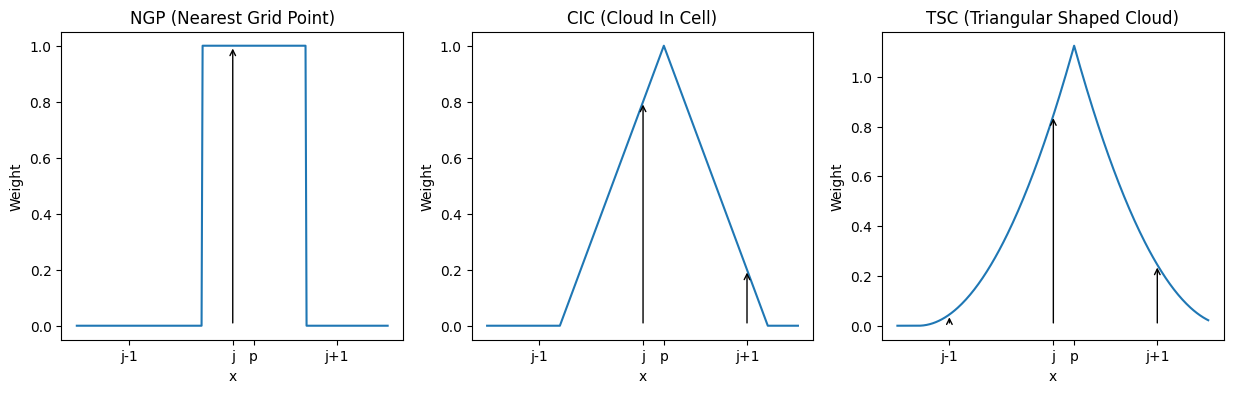
\includegraphics[width=\textwidth]{figures/weight_functions.png}
    \caption[Illustration of three mass assignment schemes]{Illustration of three mass assignment schemes—Nearest Grid Point (NGP), Cloud-In-Cell (CIC), and Triangular-Shaped Cloud (TSC)—used to map a particle's mass onto a 1D grid.}
    \label{fig:mass-assignment}
\end{figure}

\subsection{Parallelization Techniques}
Parallelization accelerates computations in large-scale simulations by leveraging multiple processors or computing nodes. Key strategies include:
\begin{itemize}
    \item \textbf{Domain Decomposition:} The computational domain is partitioned into smaller subdomains, each assigned to a separate processor \citep{1986Natur.324..446B}.
    \item \textbf{Task Parallelism:} Distributing independent tasks across multiple processors.
    \item \textbf{Data Parallelism:} Performing identical operations concurrently on different data elements, enabling SIMD (Single Instruction, Multiple Data) execution.
\end{itemize}

\subsection{Adaptive Mesh Refinement}
Adaptive Mesh Refinement (AMR) dynamically adjusts grid resolution, refining the mesh where higher accuracy is needed (e.g., regions with high density gradients) and coarsening it elsewhere \citep{1989JCoPh..82...64B}. This technique is typically used in hydrodynamical simulations to capture complex fluid dynamics and shock fronts accurately.
Because N-body simulations with discrete particles do not require continuous field solution and have more efficient methods like Tree-PM, AMR is not commonly used in N-body simulations.

This creates a hierarchy of grids with increasing resolution and optimizes computational resources. Refinement is typically triggered when: 
\begin{equation}
    \left| \nabla \phi(\mathbf{x}) \right| > \theta,
\end{equation}
with $\theta$ being a predefined threshold.

\begin{figure}
    \centering
    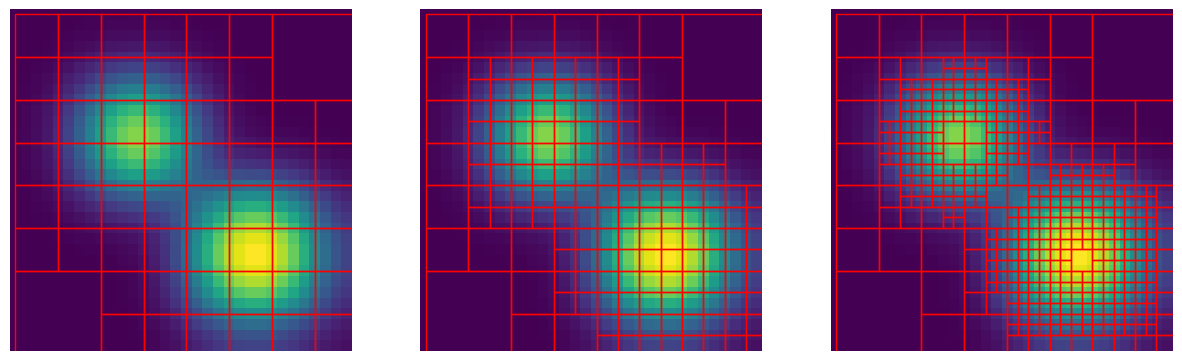
\includegraphics[width=\textwidth]{figures/adaptive_mesh_refinement.png}
    \caption[Illustration of adaptive mesh refinement]{Illustration of adaptive mesh refinement (AMR) applied to a 2D image with two Gaussian kernels. The left panel shows the initial coarse grid structure over the image. The middle and right panels demonstrate progressively finer levels of mesh refinement in regions of higher intensity, where the Gaussian kernels are located. The red grid outlines indicate the adaptively refined mesh hierarchy, ensuring higher resolution where needed while maintaining computational efficiency in lower-intensity regions.}
    \label{fig:amr}
\end{figure}
Figure~\ref{fig:amr} demonstrates the application of Adaptive Mesh Refinement (AMR) to a two-dimensional image containing two Gaussian kernels. Initially, a uniformly coarse grid overlays the entire image (left panel). As the refinement process progresses, the mesh becomes increasingly finer in regions with higher intensity, specifically around the Gaussian kernels (middle and right panels). The red grid lines represent the hierarchy of the refined meshes, enabling higher resolution where it is most needed and optimizing computational resources by keeping a coarser grid in less significant areas.

\subsection{Tree Construction}
Tree-based data structures efficiently organize hierarchical spatial data. The Barnes-Hut algorithm employs an octree to partition space, reducing computational complexity from $\mathcal{O}(N^2)$ to $\mathcal{O}(N \log N)$ by approximating distant particle clusters as single mass points. This approximation is controlled by the opening angle $\theta$:
\begin{equation}
    \frac{s}{d} < \theta,
\end{equation}
where $s$ is the node size and $d$ is the distance from the particle to the node's center of mass.

One of the popular algorithms for tree construction is the Barnes-Hut Octree \citep{1986Natur.324..446B}, which recursively subdivides the simulation volume into hierarchical grid cells. Figure~\ref{fig:barnes-hut} illustrates the Octree decomposition for a 3D volume containing four particles.
\begin{figure}[ht]
    \centering
    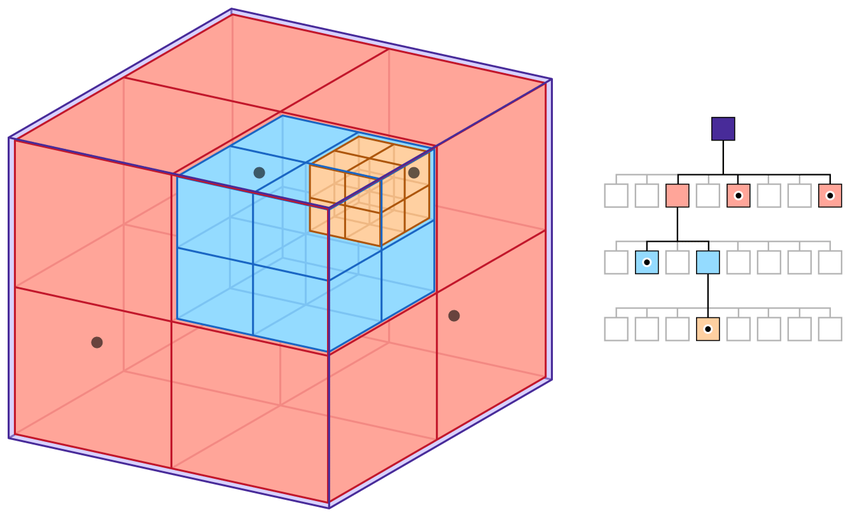
\includegraphics[width=0.6\textwidth]{figures/Octree.png}
    \caption[Illustration of an Octree decomposition]{Illustration of an Octree decomposition for a 3D volume containing four particles. The left panel showcases the spatial subdivision of the volume into hierarchical grid cells, with color-coding indicating different levels of refinement. The right panel presents the corresponding Octree data structure, highlighting the hierarchical relationships between nodes. Credit by \citet{Powell2023}}
    \label{fig:barnes-hut}
\end{figure}

Parallel tree construction involves building local trees within each subdomain and integrating them for global computations \citep{DUBINSKI1996133}. Efficient parallelization enhances scalability and performance in large-scale simulations.

\section{\texttt{FASTPM}} \label{sec:fastpm}
\texttt{FASTPM} (Fast Particle Mesh; \citealt{10.1093/mnras/stw2123}) is an advanced N-body simulation code tailored for efficiently modeling the evolution of dark matter and halo structures on cosmological scales. Building upon the foundational PM approach, \texttt{FASTPM} integrates modified kick and drift factors derived from the Zel'dovich Approximation (ZA). This enhancement allows \texttt{FASTPM} to achieve high accuracy in large-scale structure formation while significantly reducing computational overhead. This subsection delineates the core methodology of FASTPM, incorporating the mathematical formalism of its modified kick and drift factors.

\subsection{Modified Kick and Drift Factors}
The cornerstone of \texttt{FASTPM}'s enhanced performance lies in its \textbf{modified kick ($K_{\text{FASTPM}}$)} and \textbf{drift ($D_{\text{FASTPM}}$)} factors. These factors are meticulously derived from the Zel'dovich Approximation (ZA), a first-order Lagrangian perturbation theory (1LPT), to rectify inaccuracies in large-scale growth inherent in standard PM solvers, especially when operating with a limited number of time steps.

First, the Zel'dovich equation of motion to the first order is defined as:
\begin{eqnarray}
    \mathbf{x}_{\text{ZA}}(a) &=& \mathbf{q} + D(a)\mathbf{s}_1,  \nonumber \\
    \mathbf{p}_{\text{ZA}}(a) &=& a^3 E(a) g_p(a) \mathbf{s}_1,  \nonumber \\
    \mathbf{f}_{\text{ZA}}(a) &=& a^2 E(a) g_f(a) \mathbf{s}_1, 
\end{eqnarray}
where $E(a) = \frac{H(a)}{H(a=1)}$ is the dimensionless Hubble parameter, and $g_p(a)$ and $g_f(a)$ are auxiliary factors defined as:
\begin{eqnarray}
    g_p(a)  &=& \frac{dD}{da},  G_p(a) = D(a) \\[0.5em]
    g_f(a)  &=& \frac{d(a^3 E g_p)}{da}, G_f(a) = a^3 E g_p(a)
\end{eqnarray}
The ZA equations of motion are reformulated in terms of drift and kick operators by integrating over a time step from $a_0$ to $a_1$ and eliminating the ZA displacement $\mathbf{s}_1$:
\begin{eqnarray}
    \Delta \mathbf{x}_{\text{ZA}} &=& \mathbf{x}_{\text{ZA}}(a_1) - \mathbf{x}_{\text{ZA}}(a_0) \nonumber \\
    &=& \left[ D(a) \right]_{a_0}^{a_1} \mathbf{s}_1 \nonumber \\
    &=& \frac{\mathbf{p}_{\text{ZA}}(a_r)}{a_r^3 E(a_r)} \left( \frac{\Delta G_p}{g_p(a_r)} \right),
\end{eqnarray}
\begin{eqnarray}
    \Delta \mathbf{p}_{\text{ZA}} &=& \mathbf{p}_{\text{ZA}}(a_1) - \mathbf{p}_{\text{ZA}}(a_0) \nonumber \\
    &=& \frac{\mathbf{f}_{\text{ZA}}(a_r)}{a_r^2 E(a_r)} \left( \frac{\Delta G_f}{g_f(a_r)} \right),
\end{eqnarray}
where $\Delta \mathbf{x}_{\text{ZA}}$ is the change in displacement over the time step, $\Delta \mathbf{p}_{\text{ZA}}$ is the change in momentum over the time step, $a_r$ is a reference scale factor within the time step, $\Delta G_p = G_p(a_1) - G_p(a_0)$, and $\Delta G_f = G_f(a_1) - G_f(a_0)$.
Therefore, the modified kick and drift factors in FASTPM are defined as:
\begin{eqnarray}
    \mathcal{D}_{\text{FASTPM}} &=& \frac{\Delta \mathbf{x}_{\text{ZA}}}{\mathbf{p}_{\text{ZA}}} 
        = \frac{1}{a_r^3 E(a_r)} \left( \frac{\Delta G_p}{g_p(a_r)} \right) \\[1em]
    \mathcal{K}_{\text{FASTPM}} &=& \frac{\Delta \mathbf{p}_{\text{ZA}}}{\mathbf{f}_{\text{ZA}}} 
        = \frac{1}{a_r^2 E(a_r)} \left( \frac{\Delta G_f}{g_f(a_r)} \right) 
\end{eqnarray}
These operators ensure the exact integration of the ZA equations of motion, thereby accurately capturing the linear growth of structures within each time step.

\subsection{Algorithm Steps}
The main steps of the \texttt{FASTPM} algorithm follow the standard PM method discussed in Section~\ref{sec:pm-method}, with the addition of the modified kick and drift operators to ensure accurate linear growth.

\begin{enumerate}
    \item \textbf{Apply Modified Operators:}
    \label{fastpm:modified-kick-drift}
    Utilize the modified kick ($K_{\text{FASTPM}}$) and drift ($D_{\text{FASTPM}}$) factors to update particle velocities and positions. These factors, derived from the ZA, ensure accurate linear growth:
    
    \begin{enumerate}
        \item \textbf{Kick Step:}
        Update particle velocities by applying the gravitational acceleration scaled by the modified kick factor:
        \[
        \mathbf{v}_i\left(t + \frac{\Delta t}{2}\right) = \mathbf{v}_i(t) + \mathbf{g}_i(t) \cdot K_{\text{FASTPM}} \cdot \Delta t
        \]
        
        \item \textbf{Drift Step:}
        Update particle positions using the updated velocities and the modified drift factor:
        \[
        \mathbf{r}_i(t + \Delta t) = \mathbf{r}_i(t) + \mathbf{v}_i\left(t + \frac{\Delta t}{2}\right) \cdot D_{\text{FASTPM}} \cdot \Delta t
        \]
        
        \item \textbf{Second Kick Step:}
        Apply another kick to update velocities to the full time step:
        \[
        \mathbf{v}_i(t + \Delta t) = \mathbf{v}_i\left(t + \frac{\Delta t}{2}\right) + \mathbf{g}_i(t + \Delta t) \cdot K_{\text{FASTPM}} \cdot \Delta t
        \]
    \end{enumerate}
    
    \item \textbf{Update Particle States:}
    Finalize the update of particle velocities and positions after applying the modified kick and drift operators:
    \[
    \mathbf{v}_i(t + \Delta t) = \mathbf{v}_i\left(t + \frac{\Delta t}{2}\right) + \mathbf{g}_i(t + \Delta t) \cdot K_{\text{FASTPM}} \cdot \Delta t
    \]
    \[
    \mathbf{r}_i(t + \Delta t) = \mathbf{r}_i(t) + \mathbf{v}_i\left(t + \frac{\Delta t}{2}\right) \cdot D_{\text{FASTPM}} \cdot \Delta t
    \]
    
    \item \textbf{Advance Time:}
    Increment the simulation time by the time step $\Delta t$:
    \[
    t \leftarrow t + \Delta t
    \]
\end{enumerate}

\section{Weak Lensing Map Generation}
\label{sec:weak-lensing-generation}
To extract statistics from N-body simulations, it is necessary to generate detailed WL maps by simulating the propagation of a vast number of virtual light rays from source galaxies to the observer. This process involves calculating the distortions and magnifications of the source images caused by the cumulative gravitational deflections from the intervening matter distribution along each line of sight.

\subsection{Conventional Ray-Tracing Algorithm}
\label{subsec:conventional-ray-tracing}
Conventional ray-tracing algorithms are fundamental tools for generating WL maps from N-body simulations. These algorithms simplify the complex three-dimensional matter distribution by projecting it onto a series of two-dimensional lens planes. The numerical implementation of the ray-tracing algorithm involves several key computational steps, outlined below \citep{2008ApJ...682....1D, 2009A&A...497..335T, 2015MNRAS.453.3043S}:

\begin{enumerate}
    \item \textbf{Lens Plane Generation:} 
    The first step involves constructing the surface mass density $\Delta_\Sigma^j(\boldsymbol{\theta})$ for each lens plane $j$. This is achieved by projecting the three-dimensional matter density $\rho(\chi, \chi\boldsymbol{\theta})$ within a spherical shell bounded by comoving distances $\chi_j$ and $\chi_{j+1}$ onto a two-dimensional plane:
    \begin{equation}
        \Delta_\Sigma^j(\boldsymbol{\theta}) = \int_{\chi_j}^{\chi_{j+1}} \left[ \rho(\chi, \chi\boldsymbol{\theta}) - \bar{\rho}(\chi) \right] \chi^2 \, \mathrm{d}\chi,
    \end{equation}
    where $\bar{\rho}(\chi)$ is the mean matter density at distance $\chi$. 
    The effective comoving distance to the center of the $j$-th shell, $\chi^j$, is calculated as \citep{2015MNRAS.453.3043S}:
    \begin{equation}
        \chi^j = \frac{\int_{\chi_{\min}}^{\chi_{\max}} \chi^3 \, \mathrm{d}\chi}{\int_{\chi_{\min}}^{\chi_{\max}} \chi^2 \, \mathrm{d}\chi} = \frac{3}{4} \frac{\chi_{\max}^4 - \chi_{\min}^4}{\chi_{\max}^3 - \chi_{\min}^3},
    \end{equation}
    where $\chi_{\min}$ and $\chi_{\max}$ are the minimum and maximum comoving distances of the shell, respectively.
    The convergence field $\kappa_j(\boldsymbol{\theta})$ for the $j$-th lens plane is then computed as:
    \begin{equation}
        \kappa_j(\boldsymbol{\theta}) = \frac{4\pi G}{c^2} \frac{\Delta_\Sigma^j(\boldsymbol{\theta})}{a_j \chi_j},
    \end{equation}
    with $a_j$ being the scale factor and $\chi_j$ the comoving distance to the $j$-th lens plane.

    To express $\kappa_j(\boldsymbol{\theta})$ in terms of the simulation parameters, we consider the following quantities:
    \begin{itemize}
        \item $V_{\mathrm{sim}}$: The simulation volume.
        \item $N_{\mathrm{part}}$: The total number of particles in the simulation.
        \item $N_{\mathrm{pix}}$: The number of pixels on each lens plane.
        \item $n_{\mathrm{part}}^j$: The number of particles in the $j$-th shell.
        \item $\bar{n}_{\mathrm{part}}^j$: The mean number of particles per pixel in the $j$-th shell.
    \end{itemize}
    The convergence field is then given by:
    \begin{equation}
        \kappa_j(\boldsymbol{\theta}) = \frac{3H_0^2\Omega_m}{2c^2 a_j \chi_j} \frac{V_{\mathrm{sim}}}{N_{\mathrm{part}}} \frac{N_{\mathrm{pix}}}{4\pi} \left( n_{\mathrm{part}}^j - \bar{n}_{\mathrm{part}}^j \right),
    \end{equation}

    \item \textbf{Potential Calculation:} 
    To facilitate the computation of lensing effects, the lensing potential $\psi^j(\boldsymbol{\theta})$ for each lens plane is derived from the convergence field $\kappa_j(\boldsymbol{\theta})$. This is efficiently done using spherical harmonics:
    \begin{equation}
        \psi_{lm}^j = \frac{2}{l(l+1)} \kappa_{lm}^j \quad \text{for} \quad l \neq 0,
    \end{equation}
    and $\psi_{lm}^j = 0$ for $l = 0$. Subsequently, the lensing potential in real space is reconstructed, allowing the calculation of the deflection field $\boldsymbol{\alpha}^j(\boldsymbol{\theta})$ and the optical tidal matrix $U_{ik}^j(\boldsymbol{\theta})$ through:
    \begin{equation}
        \alpha_i^j = -\nabla_i \psi^j, \quad U_{ik}^j = \nabla_i \nabla_k \psi^j.
    \end{equation}

    \item \textbf{Deflection Angle Determination:} 
        The deflection field $\boldsymbol{\alpha}^j(\boldsymbol{\theta})$ and the optical tidal matrix $U_{ik}^j(\boldsymbol{\theta})$ are interpolated to arbitrary positions on each lens plane. The lensing matrix $\mathcal{A}^j_{ik}$ at each plane is then updated using the recurrence relation:
        \begin{equation}
            \begin{aligned}
                \mathcal{A}_{i k}^{j+1} & = \left(1 - \frac{\chi_j}{\chi_{j+1}} \frac{\chi_{j+1} - \chi_{j-1}}{\chi_j - \chi_{j-1}} \right) \mathcal{A}_{i k}^{j-1} + \frac{\chi_j}{\chi_{j+1}} \frac{\chi_{j+1} - \chi_{j-1}}{\chi_j - \chi_{j-1}} \mathcal{A}_{i k}^j \\
                & \quad - \frac{\chi_{j+1} - \chi_j}{\chi_{j-1}} U_{i m}^j \mathcal{A}_{m k}^j,
            \end{aligned}
        \end{equation}
        with the initial conditions:
        \begin{equation}
            \mathcal{A}_{i k}^1 = \delta_{i k}, \quad \mathcal{A}_{i k}^0 = \delta_{i k},
        \end{equation}
    for $j \geq 1$. The closest lens plane to the observer is designated as $j = 0$.

    \item \textbf{Ray Propagation:} 
    Light rays are propagated from the source galaxies to the observer through the sequence of lens planes. At each plane, the accumulated deflection angles are updated based on the lensing matrix $\mathcal{A}^j_{ik}$. 

    \item \textbf{Map Assembly:} 
    After propagating all light rays through the lens planes, the convergence $\kappa(\boldsymbol{\theta})$ and shear $\gamma(\boldsymbol{\theta})$ fields are compiled into full-sky maps, using Eq.~\eqref{eq:jacobian_matrix}. These maps are typically represented on the \texttt{HEALPix} grid.
\end{enumerate}

\subsection{Born-approximated Ray-tracing}
The Born approximation offers a simplified approach to weak lensing map generation by assuming that light rays travel along their unperturbed, straight-line paths from the source galaxies to the observer. This approximation neglects the bending of light rays due to gravitational deflections between lens planes, thereby reducing the computational complexity of the ray-tracing process \citep{2006glsw.conf..269S}. 

While this simplification can lead to faster computations, it introduces certain limitations in accurately capturing multiple deflections and non-linear lensing effects. 
To overcome these limitations, researchers have developed Post-Born corrections \citep{2002ApJ...574...19C, 2005PhRvD..72j3004D} that account for the deflection during ray propagation and for the so-called lens-lens coupling, which describes how gravitational lenses at different redshifts can interact to generate rotational modes in the observable fields. It is shown that the Post-Born corrections can impact the higher-order moments or peak statistics of galxy weak lensing convergence maps \citep{2017PhRvD..95l3503P, 2019JCAP...10..057F}. Figure~\ref{fig:born-approximation} \citep{2017PhRvD..95l3503P} illustrates the parameter bias induced by the Born approximation in the convergence power spectrum and moments of the convergence field. The Born approximation is accurate in predicting the convergence power spectrum, but it leads to significant biases in the moments of the convergence field.

\begin{figure}[ht]
    \centering
    \begin{subfigure}[b]{0.48\textwidth}
        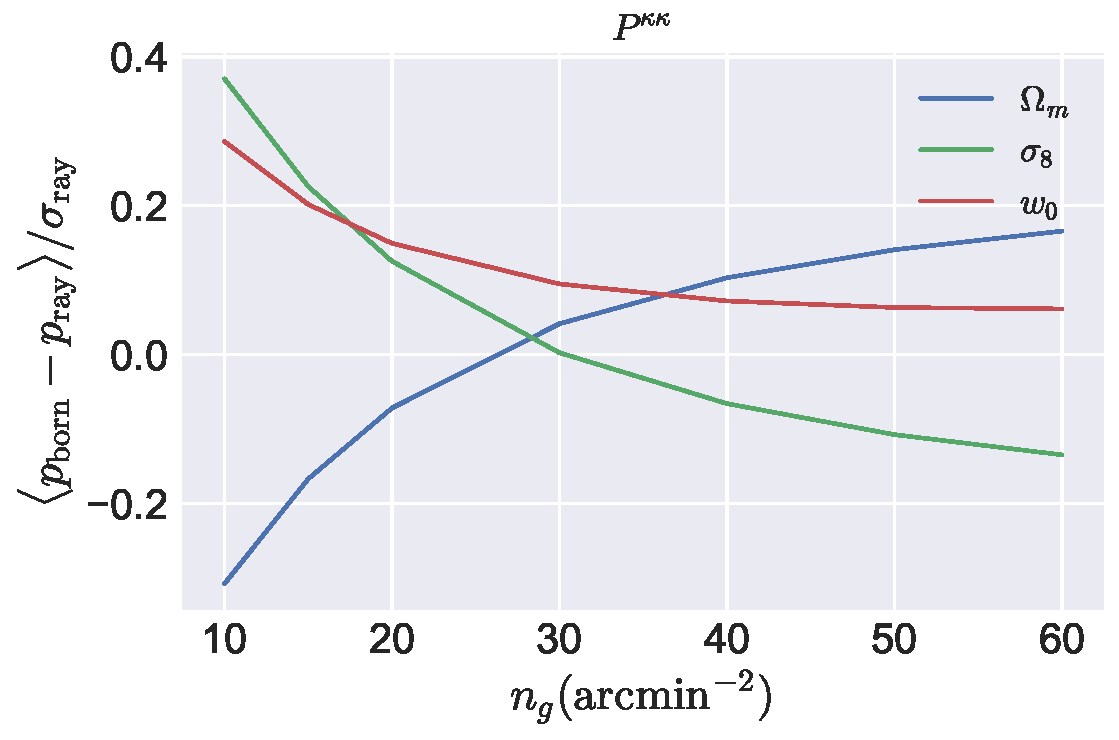
\includegraphics[width=\textwidth]{figures/bias_ngal_convergence_powerSN_s0_nb100.pdf}
    \end{subfigure}
    \hfill
    \begin{subfigure}[b]{0.48\textwidth}
        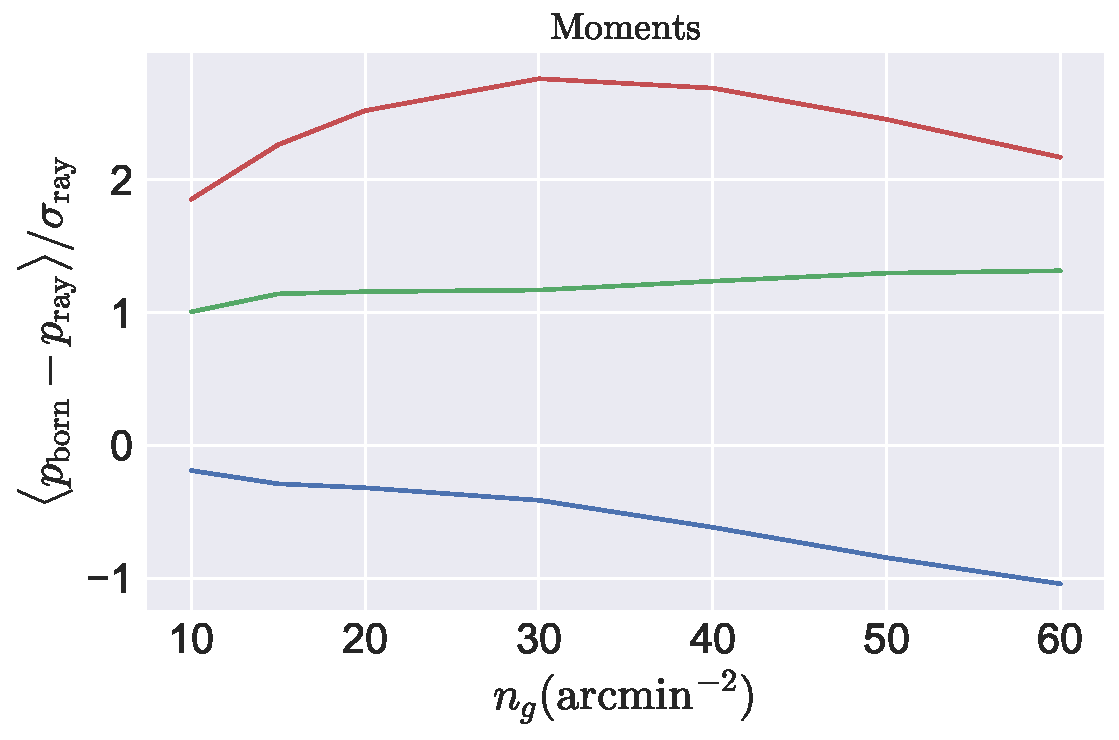
\includegraphics[width=\textwidth]{figures/bias_ngal_convergence_momentsSN_s50_nb9.pdf}
    \end{subfigure}
    \caption[Parameter bias induced by the Born approximation]{Parameter bias induced by the Born approximation in the convergence power spectrum (Left Panel) and moments of the convergence field (Right Panel). While the Born approximation is accurate in predicting the convergence power spectrum, it leads to significant biases in the moments of the convergence field. credit by \citet{2017PhRvD..95l3503P}}
    \label{fig:born-approximation}
\end{figure}

Nonetheless, the Born-approximation remains a valuable tool for generating weak lensing maps in large-scale structure studies \citep{2008MNRAS.391..435F, 2009A&A...499...31H, 2015MNRAS.447.1319F}.
The Born-approximated ray-tracing algorithm comprises the following key steps:

\begin{enumerate}
    \item \textbf{Lens Plane Calculation:} 
    For each lens plane $j$, the convergence contribution $\kappa_j(\boldsymbol{\theta})$ is computed independently, incorporating the lensing efficiency function $W(\chi_j, \chi_s)$, where $\chi_j$ is the comoving distance to the $j$-th lens plane and $\chi_s$ is the comoving distance to the source galaxy. The convergence on the $j$-th plane is given by
    \begin{equation}
        \kappa_j(\boldsymbol{\theta}) = W(\chi_j, \chi_s) \delta_j(\boldsymbol{\theta}) \Delta \chi_j,
        \label{eq:kappa_born}
    \end{equation}
    where $\delta_j(\boldsymbol{\theta}) = n_{\mathrm{part}}^j(\boldsymbol{\theta}) / \bar{n}_{\mathrm{part}}^j - 1$ represents the projected matter density contrast on the $j$-th lens plane, and $\Delta \chi_j$ is the comoving thickness of the $j$-th lens plane. The lensing efficiency function, previously defined in Eq.~\eqref{eq:lensing_efficiency_flat}, is discreditized for each lens plane as:
    \begin{equation}
        W(\chi_j, \chi_s) = \frac{3 H_0^2 \Omega_m}{2 c^2} \frac{( \chi_s - \chi_j )}{ \chi_s } \frac{ \chi_j }{ a_j },
    \end{equation}

    \item \textbf{Convergence Field Assembly:} 
    The total convergence field $\kappa(\boldsymbol{\theta})$ is obtained by summing the contributions from all individual lens planes:
    \begin{equation}
        \kappa(\boldsymbol{\theta}) = \sum_{j} \kappa_j(\boldsymbol{\theta}).
        \label{eq:total_kappa}
    \end{equation}
    This linear superposition is a direct consequence of the Born approximation, which assumes that each lens plane contributes independently to the total convergence without accounting for the altered path of the light ray due to previous deflections.

\end{enumerate}
